% Chapter 2 -- structure from table of content.md; impersonal academic style

\reportchapter{1}{Project Context and Requirements}{}

\section{Introduction}

This chapter presents the institutional and operational context of the project. It introduces SCIENTIAE and its research need, defines the problem and objectives, presents the proposed solution, identifies actors and requirements, explains the principal UML models, justifies the selected technology stack, and describes the project-management approach. Chapter~2 then provides the state of the art supporting these choices.

\section{Host Organization}

\subsection{Company Profile and Activities}

The project was carried out at \textbf{SCIENTIAE}, a technology company based in Rabat whose activities cover software engineering, data science, cybersecurity, and the development of decision-support solutions. The company favors open and controlled infrastructure so that sensitive data, processing services, and analytical results can remain under organizational governance.

\begin{figure}[H]
    \centering
    
\includegraphics[height=1.5cm]{Logos/Company_Logo_Scientiae.png}
    \caption{SCIENTIAE, host organization of the project.}
    \label{fig:host-organization}
\end{figure}

As illustrated in Figure~\ref{fig:org-chart}, SCIENTIAE operates under the direction of its General Management and is organized into two principal departments. The \textbf{Administrative Department} brings together the Human Resources and Finance functions, which support personnel administration and the company's financial operations. The \textbf{Research and Development Department} concentrates the company's technical and innovation activities through three complementary teams: Cybersecurity Engineering, Software Engineering, and Data Science Engineering.

\begin{figure}[H]
    \centering
    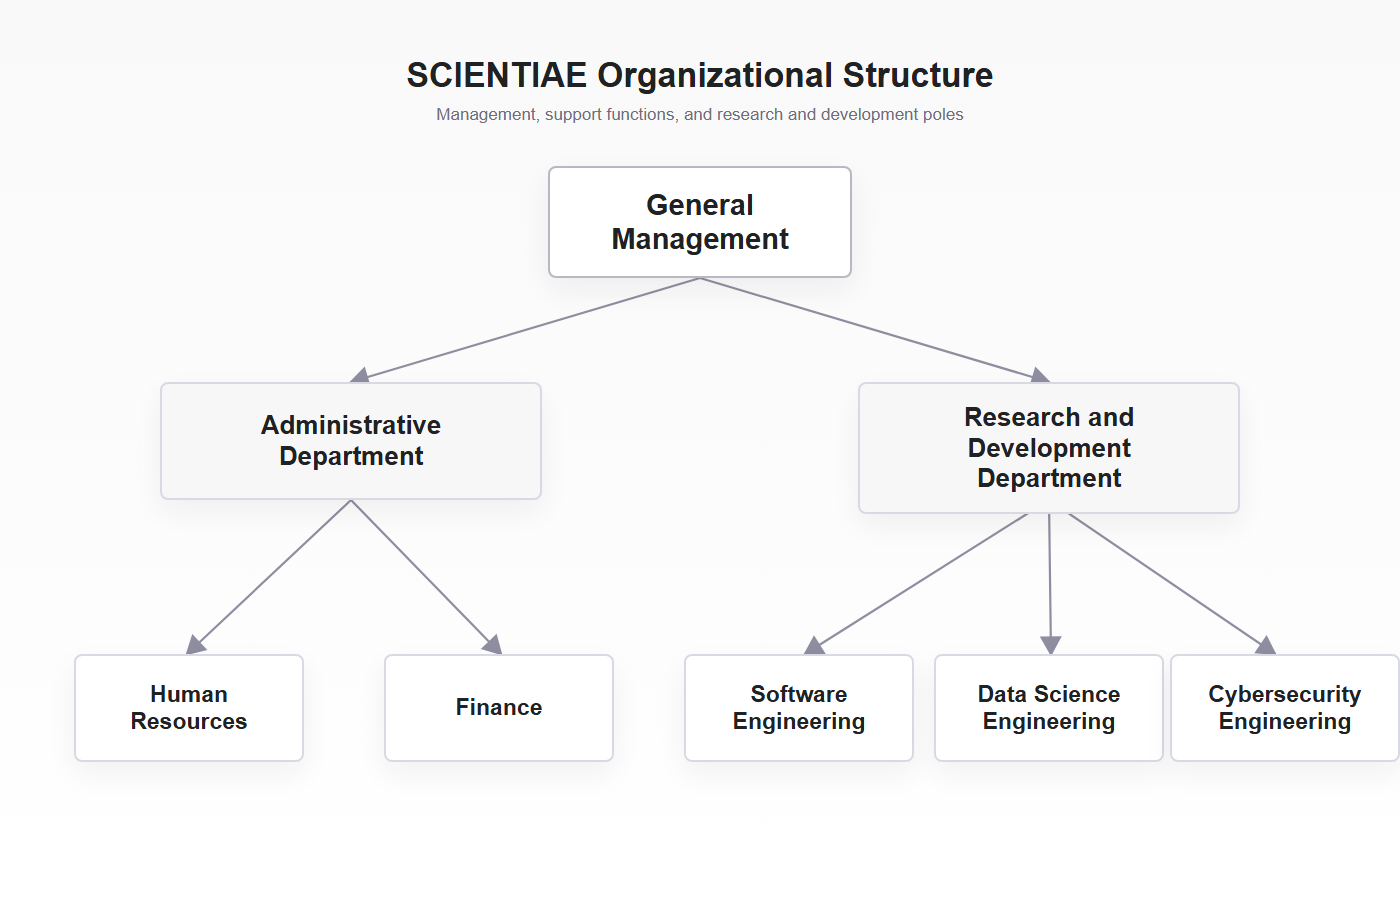
\includegraphics[width=\textwidth,height=0.78\textheight,keepaspectratio]{images/org_chart.png}
    \caption{Organizational structure of SCIENTIAE.}
    \label{fig:org-chart}
\end{figure}

The project was carried out within the \textbf{Data Science Engineering team} of the Research and Development Department, highlighted in the organizational chart. This position placed the work at the intersection of data engineering, natural language processing, knowledge representation, information retrieval, and generative artificial intelligence. The team provided the appropriate environment for researching and implementing a Graph-RAG framework capable of collecting heterogeneous information, extracting entities and relations, constructing knowledge graphs, and producing evidence-grounded answers.

Although the political and geopolitical domain was selected for implementation and validation, the work contributes to SCIENTIAE's broader R\&D objective of developing reusable and sovereign AI-based decision-support solutions. Collaboration with the Software Engineering team supported the integration of backend services and the analytical interface, while the wider R\&D structure ensured that concerns such as system security, controlled infrastructure, maintainability, and deployment were considered throughout the project.

\subsection{Research Need}

Within its R\&D activities, SCIENTIAE is developing a sovereign Graph-RAG framework intended to adapt to multiple domains. The objective is to establish reusable acquisition, extraction, graph-construction, retrieval, reasoning, and evaluation components whose domain-specific elements---sources, ontology, prompts, and validation questions---can be configured without redesigning the complete platform.

Politics and geopolitics were selected as the application and validation domain because they combine heterogeneous sources, ambiguous actors, evolving facts, multi-hop relationships, and strict traceability needs. This domain provides a demanding test of whether the framework can transform unstructured information into connected, current, and inspectable knowledge.

\section{Problem Definition}

\subsection{Core Problem Statement}

Political intelligence analysis increasingly depends on relational questions. An analyst may need to determine how two actors are connected, which events explain a diplomatic shift, how an institution evolved over time, or which documents support a specific claim. These questions cannot be answered robustly when documents are treated as isolated text fragments. They require a representation that combines textual evidence with structured relations, temporal context, and explicit source attribution.

The modern geopolitical landscape generates a volume of unstructured data that exceeds manual monitoring capacity. Analysts must follow hundreds of heterogeneous sources while preserving traceability from generated statements back to original evidence. Traditional keyword search retrieves documents but does not resolve entity ambiguity or traverse typed relationships. Classical retrieval-augmented generation can summarize passages but remains weak on multi-hop reasoning, temporal consistency, and auditable citations.

The platform developed during this end-of-study internship must therefore support four core capabilities: relational traversal across multi-hop chains of influence; contextual grounding through granular, citable evidence; synthesis of coherent answers with attribution; and architectural flexibility to adapt the same pipeline to evolving source registries and analytical domains. A representative query illustrates the difficulty: identifying the indirect diplomatic consequences of a legislative vote in one country on bilateral relations with another requires structured traversal rather than flat chunk retrieval alone.

\subsection{Scope and Constraints}

The project scope covers the end-to-end workflow from autonomous acquisition of public political documents to grounded question answering over a hybrid vector-and-graph store. The initial corpus targets \textbf{57 distinct and expandable international sources}, with ingestion extended through RSS monitoring, query-driven news discovery, direct URL submission, and PDF report parsing. Out of scope for the core deliverable are proprietary closed datasets unavailable for ingestion, real-time social-media firehose processing at web scale, and fully automated judgment of legal or normative correctness beyond evidence-backed synthesis.

Engineering constraints include dependence on external LLM APIs for extraction and answer generation, finite GPU and token budgets during development, and the need to operate on sovereign or locally controlled infrastructure for sensitive corpora. The pipeline must remain modular so that crawling, extraction, indexing, retrieval, and evaluation can be executed and inspected independently. These constraints shape the requirements listed in the following sections and are revisited in the design and implementation chapters.

\subsection{Target Domain Assumptions}

The primary domain assumption is that relevant political evidence appears in public or semi-structured textual sources---news articles, institutional reports, RSS entries, and policy PDFs---rather than in a pre-built external knowledge base. Entity mentions are noisy, syndicated, and temporally evolving; the same actor may appear under multiple surface forms, and facts may change over time. The system therefore assumes that entity resolution, temporal metadata, and provenance preservation are first-class requirements rather than optional enrichments.

A second assumption is that analysts require both conversational access and direct inspection of underlying artifacts: source documents, graph neighborhoods, ingestion status, and reasoning traces. A third assumption is domain adaptability at the pipeline level: the ingestion layer remains broad while extraction schemas and graph ontologies can be refined without rewriting the frontend or storage interfaces. These assumptions motivate the hybrid retrieval architecture proposed in this project and are examined against the state of the art in Chapter~2.

\section{Proposed Solution and Objectives}

\subsection{Solution Overview}

The proposed solution is a modular multimodal Graph-RAG framework instantiated for political and geopolitical analysis. It autonomously collects public information, normalizes and stores source documents, extracts entities and relations, constructs a knowledge graph, indexes textual chunks for semantic search, and combines graph and vector evidence to generate cited answers. An analytical interface exposes conversational questioning, source inspection, graph exploration, specialized dashboards, and administrative supervision.

The political implementation is both a usable decision-support platform and a validation environment for the broader framework. Adaptation to another domain is achieved by changing source connectors, extraction schemas, ontology definitions, prompts, and evaluation benchmarks while preserving the principal service boundaries and retrieval workflow.

\subsection{Project Objectives}

\begin{itemize}[leftmargin=*, itemsep=4pt]
\item \textbf{General objective:} design and validate a sovereign Graph-RAG framework adaptable to different knowledge-intensive domains.
\item \textbf{Domain objective:} instantiate and evaluate the framework using political and geopolitical information.
\item \textbf{Data objective:} autonomously collect, normalize, deduplicate, and preserve the provenance of heterogeneous sources.
\item \textbf{Knowledge objective:} improve the reliability of LLM-based extraction during ingestion and publish stable entities, events, temporal facts, and typed relations to an inspectable knowledge graph.
\item \textbf{Reasoning objective:} combine semantic retrieval and graph traversal for factual, relational, temporal, and multi-hop questions.
\item \textbf{Trust objective:} attach citations, evidence, logs, and reasoning traces to analytical results.
\item \textbf{Engineering objective:} deliver modular, observable, testable, and deployable services with integrated user and administration interfaces.
\end{itemize}

\section{Actors and Use Cases}

\subsection{Actor Definitions}

Two primary actors interact with the platform. The \textbf{authenticated user} represents analysts, journalists, and researchers who ask cited questions in natural language, explore graph relationships, inspect documents, follow political trends, compare entities, and consult legislative or financial signals exposed by the application. The \textbf{system administrator} represents an elevated role responsible for monitoring service health, supervising users, launching and scheduling collection jobs, inspecting ingestion logs, and triggering backfill or maintenance operations on the document and vector indexes.

Both actors depend on traceability: the user must be able to verify evidence behind each answer, while the administrator must be able to verify that the corpus remains fresh, deduplicated, and processable by the extraction pipeline. These roles directly map to the functional requirements for reasoning, administration, and observability developed later in this chapter.

\subsection{Use Case Diagram Overview}

Figure~\ref{fig:use-case-diagram} provides a consolidated view of the main use cases supported by the implemented frontend and backend modules. The diagram distinguishes analytical workflows (querying, graph exploration, document consultation) from operational workflows (ingestion control, scheduler management, system monitoring).

\begin{figure}[H]
    \centering
    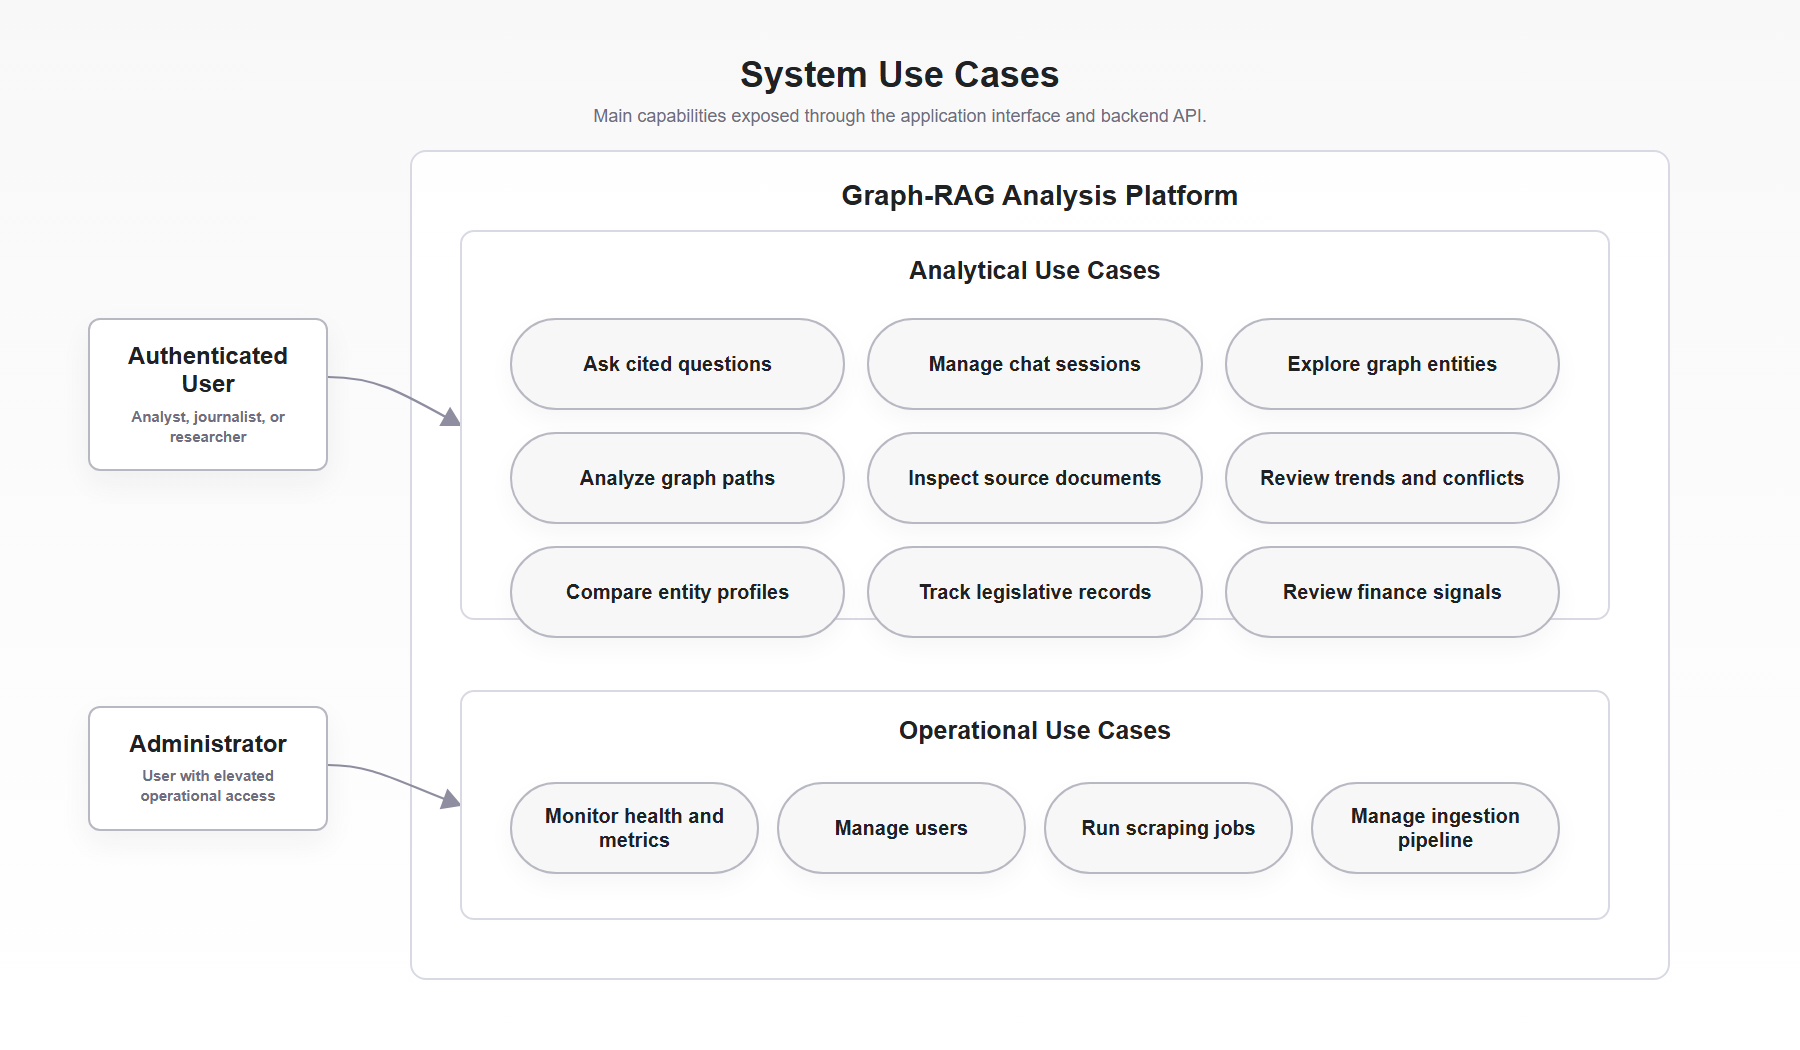
\includegraphics[width=\textwidth,height=0.82\textheight,keepaspectratio]{images/use_case_diagram.png}
    \caption{Overview of system use cases for authenticated users and administrators.}
    \label{fig:use-case-diagram}
\end{figure}

The diagram shows that query execution is not an isolated feature but part of a broader workspace that includes graph navigation, legislative and financial views, and administrative supervision. This breadth explains why requirements are grouped not only around retrieval but also around ingestion, structuring, and platform operation.

\subsection{Class Diagram Overview}

The domain class model complements the behavioral view of the use-case diagram. It identifies the principal information objects manipulated by the framework: source documents, chunks, entities, mentions, assertions, graph relations, users, sessions, and generated answers. The model also makes the provenance chain explicit, since every extracted fact and retrieved chunk remains connected to its original document.

\begin{figure}[H]
    \centering
    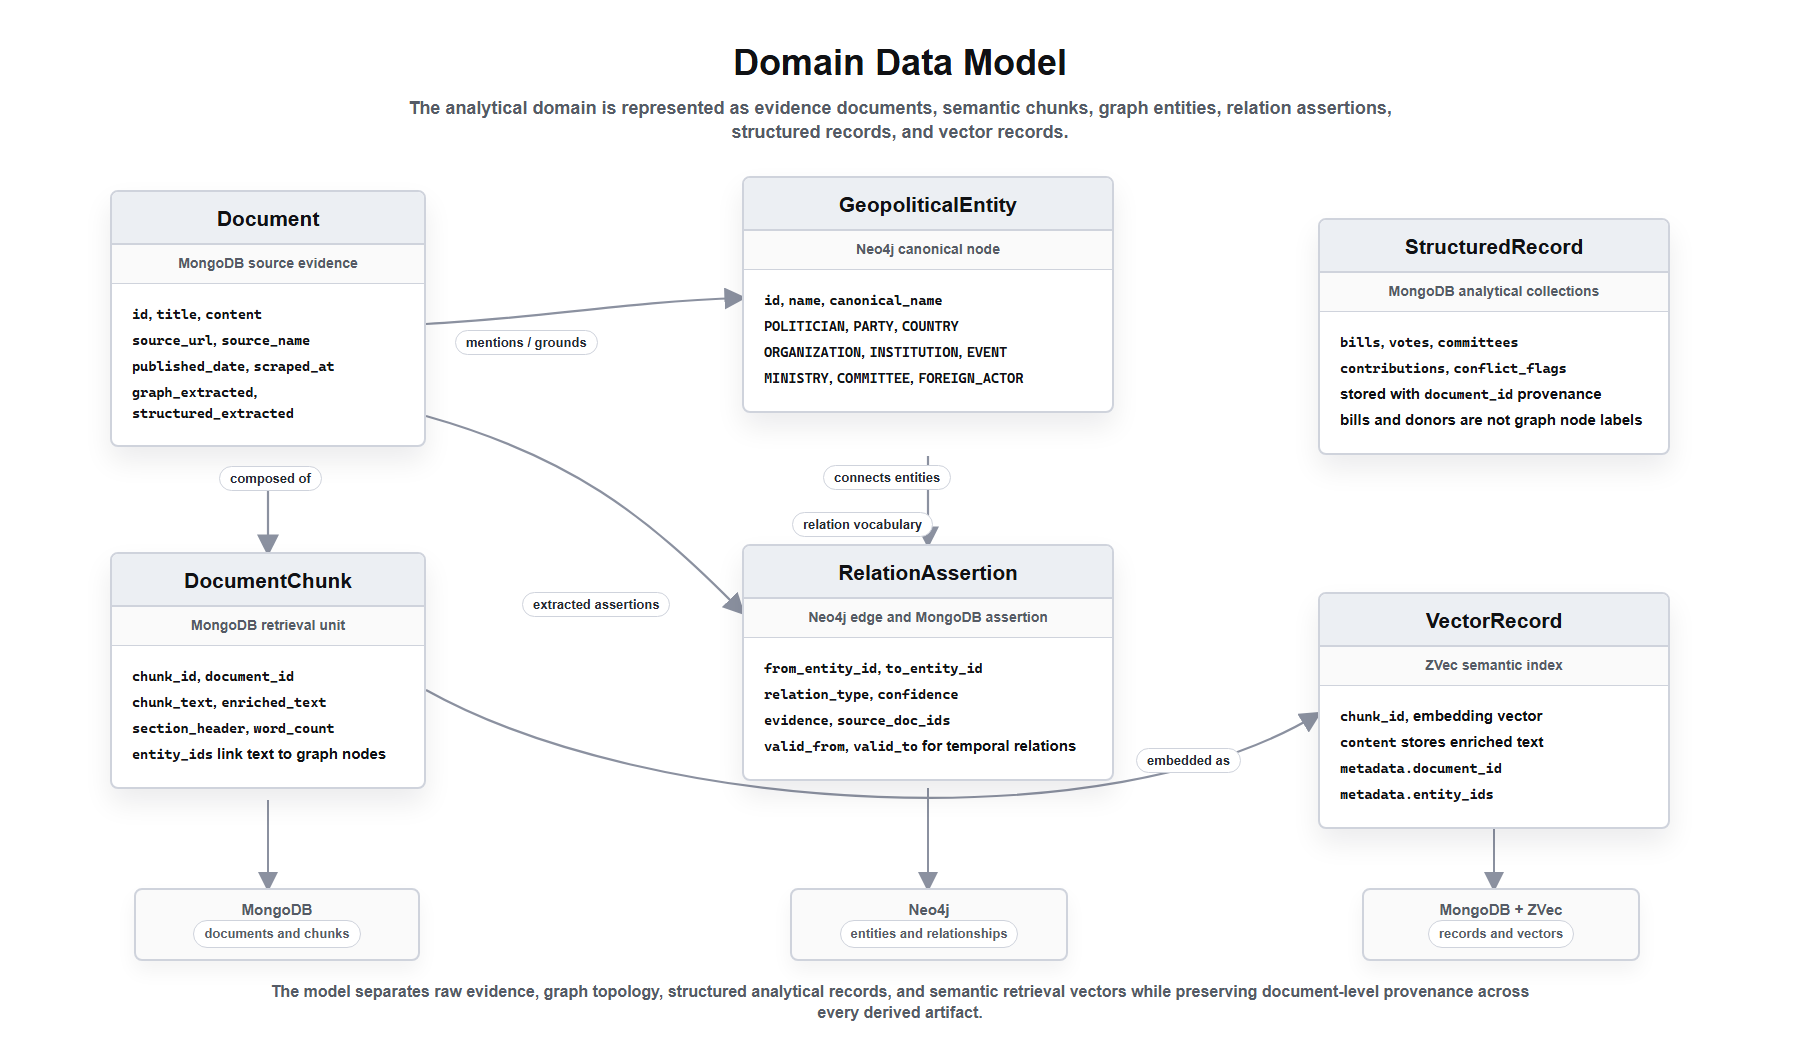
\includegraphics[width=\textwidth,height=0.82\textheight,keepaspectratio]{images/class_domain_model.png}
    \caption{UML domain class model linking documents, extracted knowledge, retrieval evidence, and user interactions.}
    \label{fig:chapter1-class-model}
\end{figure}

The class model remains conceptually reusable across domains. Domain adaptation mainly changes entity categories, relation types, and specialized structured records; document provenance, chunking, retrieval evidence, users, sessions, and answer objects remain part of the common framework.

\subsection{Key Use Case Narratives}

\newcommand{\usecasenarrative}[1]{%
  \Needspace{4\baselineskip}%
  \par\medskip\noindent #1\par
}

\usecasenarrative{\textbf{Cited analytical questioning.} An authenticated user submits a multi-hop political question through the chat interface and selects a reasoning depth (standard retrieval, decomposed multi-hop, or reflexive audit). The system retrieves semantic chunks and graph facts, synthesizes a cited answer, and exposes the reasoning trace. Success depends on grounded evidence, source links, and acceptable latency for the selected mode.}

\usecasenarrative{\textbf{Graph and document exploration.} The user inspects entity neighborhoods in the graph explorer or opens documents in the library to verify extracted relations and original wording. This use case ensures that conversational synthesis remains connected to inspectable artifacts rather than replacing them.}

\usecasenarrative{\textbf{Supervised ingestion.} An administrator triggers topic-based collection, direct URL ingestion, or scheduled scraping, then monitors logs, document counts, and index status from the administration dashboard. Failures must be visible without code changes so that corpus freshness remains under operational control.}

\usecasenarrative{\textbf{Temporal and comparative analysis.} The user consults trend, conflict, finance, or comparison views to interpret entity evolution over time. This narrative depends on temporal metadata, stable entity identifiers, and consistent graph publication after extraction.}

\section{Functional Requirements}

Functional requirements are grouped by pipeline stage. The following subsections state each requirement in full; Table~\ref{tab:functional-requirements} provides a compact registry of identifiers, short titles, and priorities without repeating the narrative descriptions.

\subsection{Data Acquisition and Ingestion}

\newcommand{\functionalrequirement}[1]{%
  \par\medskip\noindent #1\par
}

\functionalrequirement{\textbf{FR-01 (Autonomous ingestion).} The platform shall employ autonomous multi-modal ingestion capable of continuous discovery and normalization of heterogeneous political sources. Crawlers and schedulers must operate without manual reconfiguration for each new document batch, so that the corpus grows under platform control rather than through ad hoc file uploads.}

\functionalrequirement{\textbf{FR-08 (Autonomous discovery).} Collection shall extend beyond a fixed registry through LLM-guided topic expansion or administratively triggered discovery jobs. This requirement ensures that emerging sources or thematic priorities can be incorporated when analysts or supervisors identify new monitoring needs.}

\functionalrequirement{\textbf{FR-09 (Domain-agnostic ingestion).} The ingestion layer shall remain decoupled from domain-specific extraction logic. New source types, regions, or formats must be integrable by adjusting acquisition and normalization rules only, without rewriting the reasoning engine or frontend contracts.}

\functionalrequirement{\textbf{FR-10 (Heterogeneous normalization).} RSS feeds, HTML pages, direct URLs, and PDF reports shall be transformed into unified document records with consistent metadata (identifiers, timestamps, provenance, and raw text). Normalization is the prerequisite for reliable extraction and for deduplication during graph publication.}

\par\smallskip\noindent
Together, FR-01, FR-08, FR-09, and FR-10 ensure that the corpus is produced and supervised by the platform itself rather than assumed as an external input, which was identified as a central gap in Chapter~1. They directly support the \emph{supervised ingestion} use case for the administrator actor.

\subsection{Extraction and Structuring}

\functionalrequirement{\textbf{FR-02 (Joint extraction).} The system shall perform joint entity and relation extraction in a single pass over each normalized document, producing structured records aligned with the target political schema. A single-pass design reduces inconsistency between separately extracted entities and edges.}

\functionalrequirement{\textbf{FR-03 (Graph storage).} Structured outputs shall be persisted in a Neo4j knowledge graph using local deterministic entity resolution and stable canonical identifiers. Disambiguation must be reproducible so that repeated ingestion of syndicated content does not fragment one actor into multiple nodes.}

\functionalrequirement{\textbf{FR-06 (Temporal traceability).} Where publication metadata permits, the platform shall record fact evolution over time so that analysts can interpret when a relation became valid or changed. Temporal fields support trend, conflict, and comparative views described in the use-case narratives.}

\par\smallskip\noindent
Extraction quality directly conditions graph reliability and therefore constrains every downstream retrieval and reasoning function. FR-02, FR-03, and FR-06 implement the structural layer on which graph exploration and multi-hop questioning depend.

\subsection{Retrieval and Reasoning}

\functionalrequirement{\textbf{FR-04 (Hybrid search).} The platform shall combine dense vector retrieval (ZVec) with typed graph traversal (Neo4j) in a single hybrid search layer. Semantic recall over chunks and relational precision over edges must be available within the same query workflow.}

\functionalrequirement{\textbf{FR-05 (Multi-mode reasoning).} The reasoning engine shall expose three modes---standard one-hop RAG, chain-of-thought multi-hop decomposition, and reflexive agentic control---selectable at query time. Mode selection trades latency against analytical depth for the \emph{cited analytical questioning} use case.}

\functionalrequirement{\textbf{FR-07 (Attribution).} Every synthesized answer shall include a reasoning trace and precise source citations linking claims to document spans or graph facts. Attribution is mandatory for analytical trust and for jury-facing demonstration of evidence grounding.}

\functionalrequirement{\textbf{FR-11 (Automated validation).} An offline LLM-as-a-judge validation path shall support quality checks on extraction outputs and generated responses during development and evaluation (Chapter~5). This requirement does not replace human review but provides repeatable scoring hooks.}

\par\smallskip\noindent
FR-04 through FR-07 and FR-11 define the analytical core of the platform: hybrid evidence retrieval, selectable reasoning depth, auditable synthesis, and measurable quality assessment.

\subsection{User Interaction and Administration}

Beyond pipeline services, the platform shall expose an integrated frontend workspace for chat-based questioning, graph exploration, document library access, specialized political dashboards (legislative, financial, trends, conflicts, comparisons), and authenticated sessions. Administrative interfaces shall expose ingestion triggers, scheduler configuration, ingestion log inspection, and service health indicators without requiring backend code changes.

These interaction requirements implement the responsibilities of the authenticated user and system administrator defined earlier. They connect operational supervision to FR-01 and FR-08 and ensure that analytical outputs remain linked to inspectable artifacts (documents, graph neighborhoods, traces).

\begin{table}[H]
\centering
\small
\setlength{\tabcolsep}{5pt}
\renewcommand{\arraystretch}{1.35}
\begin{tabularx}{\textwidth}{@{}>{\bfseries\raggedright\arraybackslash}p{1.25cm}>{\raggedright\arraybackslash}p{2.65cm}>{\raggedright\arraybackslash}X>{\centering\arraybackslash}p{1.55cm}@{}}
\toprule
\rowcolor{lightblue}
ID & Pipeline stage & Requirement & Priority \\
\midrule
\textbf{FR-01} & Acquisition \& ingestion & Autonomous multi-modal ingestion and continuous corpus growth & High \\
\textbf{FR-08} & Acquisition \& ingestion & LLM-guided or administratively triggered source discovery & High \\
\textbf{FR-09} & Acquisition \& ingestion & Ingestion decoupled from domain-specific extraction logic & High \\
\textbf{FR-10} & Acquisition \& ingestion & Normalization of RSS, HTML, URLs, and PDFs to unified records & High \\
\textbf{FR-02} & Extraction \& structuring & Joint entity and relation extraction in a single pass & High \\
\textbf{FR-03} & Extraction \& structuring & Neo4j persistence with deterministic entity resolution & High \\
\textbf{FR-06} & Extraction \& structuring & Temporal traceability of fact evolution where applicable & High \\
\textbf{FR-04} & Retrieval \& reasoning & Hybrid ZVec vector retrieval and Neo4j graph traversal & High \\
\textbf{FR-05} & Retrieval \& reasoning & Selectable RAG, chain-of-thought, and reflexive reasoning modes & High \\
\textbf{FR-07} & Retrieval \& reasoning & Reasoning traces and precise source citations on every answer & High \\
\textbf{FR-11} & Retrieval \& reasoning & Offline LLM-as-a-judge validation for extraction and responses & High \\
\bottomrule
\end{tabularx}
\caption{Functional requirements registry.}
\label{tab:functional-requirements}
\end{table}

Table~\ref{tab:functional-requirements} confirms that every pipeline stage---from ingestion to cited synthesis---is explicitly required at high priority. Detailed component mapping appears in Chapter~3; implementation evidence appears in Chapter~4.

\section{Non-Functional Requirements}

\subsection{Performance and Scalability}

Graph traversals up to three hops should complete within approximately \textbf{500\,ms} under nominal deployment conditions so that interactive analysis remains responsive. The architecture shall support growth in document volume and graph size without proportional loss of retrieval precision. Query latency, token consumption, and throughput shall be monitorable so that optimization targets can be enforced during evaluation (Chapter~5).

\subsection{Reliability and Idempotency}

Ingestion and graph publication shall be idempotent: repeated processing of the same source URL or document identifier must not create uncontrolled duplicate nodes or bias frequency statistics. Pipeline stages shall tolerate partial failures through explicit error states, retry policies, and administrative visibility rather than silent data loss. Worker execution, caching, and proxy layers shall preserve consistent behavior under concurrent load.

\subsection{Security and Data Sovereignty}

Processing shall occur within a \textbf{sovereign infrastructure} aligned with project and host-organization constraints: local or contractually governed storage for documents, vectors, and graph data; authenticated access to analytical and administrative functions; and controlled use of external LLM APIs with documented data-handling policies. Sensitive corpora shall not depend on undisclosed third-party knowledge bases as the primary source of truth.

\subsection{Observability and Auditability}

The platform shall expose metrics, logs, and distributed traces across ingestion, retrieval, and synthesis so that bottlenecks and failures can be diagnosed in production-like conditions. Reasoning traces, citation metadata, and ingestion logs shall remain inspectable by authorized users. Observability satisfies both operational maintenance (administrator actor) and analytical trust (authenticated user actor).

\section{Technology Stack and Selection Rationale}

The stack was selected according to six criteria: compatibility with AI and data tooling, support for heterogeneous evidence, graph and vector retrieval capability, sovereignty, deployment simplicity, and maintainability. No single database is forced to represent every information type; each component is assigned the responsibility for which its data model is most appropriate.

\begin{table}[H]
\centering
\scriptsize
\renewcommand{\arraystretch}{1.25}
\begin{tabularx}{\textwidth}{@{}>{\bfseries\raggedright\arraybackslash}p{2.2cm}>{\raggedright\arraybackslash}p{2.6cm}XX@{}}
\toprule
\rowcolor{lightblue}
Layer & Selected technology & Reason for selection & Main alternative considered \\
\midrule
Backend & Python and FastAPI & Strong NLP/AI ecosystem, typed validation, asynchronous APIs, and automatic OpenAPI documentation. & Flask offers simplicity but fewer built-in typing and API-contract features. \\
Frontend & React and Vite & Component reuse, mature visualization ecosystem, fast development server, and support for an interactive analytical workspace. & Server-rendered templates are simpler but less suitable for graph and streaming interactions. \\
Document store & MongoDB & Flexible schemas for heterogeneous documents, extraction artifacts, processing states, and provenance metadata. & A relational database would require frequent schema migrations for evolving records. \\
Graph store & Neo4j & Native property-graph model, Cypher traversal, typed relationships, and mature visualization and indexing tools. & Relational joins become cumbersome for variable-depth multi-hop traversal. \\
Vector store & ZVec & Local persistent semantic retrieval with a lightweight operational footprint aligned with sovereignty requirements. & Managed vector databases provide richer scaling but add services and external dependencies. \\
LLM orchestration & Mistral and DSPy & Governed model access, structured extraction modules, and systematic optimization of knowledge extraction during ingestion. & Direct prompt calls are faster to prototype but harder to optimize and evaluate systematically. \\
Cache and streams & Redis and SSE & Low-latency temporary state and simple server-to-client streaming of reasoning progress. & WebSockets provide bidirectional communication that is unnecessary for the main response stream. \\
Deployment & Docker Compose and nginx & Reproducible local deployment, service isolation, explicit configuration, and controlled networking. & Manual installation is harder to reproduce across development and target environments. \\
Observability & Prometheus, Grafana, Jaeger & Complementary metrics, dashboards, and distributed traces for an inspectable multi-service pipeline. & Application logs alone do not explain cross-service latency or failures. \\
\bottomrule
\end{tabularx}
\caption{Technology stack and rationale for the principal engineering choices.}
\label{tab:chapter1-tech-stack}
\end{table}

\vspace{-0.45\baselineskip}
\noindent Table~\ref{tab:chapter1-tech-stack} presents the complete technology stack and the rationale behind each engineering choice. Among these components, Figure~\ref{fig:chapter1-tech-overview} highlights the representative application core. Python provides the common implementation language for ingestion, extraction, retrieval, and AI integration; FastAPI exposes these capabilities through typed asynchronous services; React delivers the interactive workspace for querying, graph exploration, and administration; and DSPy structures and optimizes the LLM-based knowledge extraction performed during ingestion. Together, these technologies connect the data and AI pipeline to a responsive user interface while preserving modularity between backend services, model orchestration, and frontend presentation.

\begin{figure}[htbp]
    \centering
    \raisebox{-0.15\height}{
\includegraphics[height=0.9cm]{Logos/python.png}}\hspace{0.5cm}
    \raisebox{-0.15\height}{
\includegraphics[height=0.9cm]{Logos/fastapi.png}}\hspace{0.5cm}
    \raisebox{-0.15\height}{
\includegraphics[height=0.9cm]{Logos/react.png}}\hspace{0.5cm}
    \raisebox{-0.15\height}{
\includegraphics[height=0.9cm]{Logos/dspy_logo.png}}
    \caption{Representative technologies used by the proposed platform.}
    \label{fig:chapter1-tech-overview}
\end{figure}

\section{Project Management}

\subsection{Validation Methodology}

Requirements were refined iteratively through user-story formulation, supervisor review, and incremental delivery of working modules. Each major function was associated with observable acceptance checks before being considered complete. Two complementary practices structured this process: \textbf{user stories}, which express stakeholder intent in testable form, and a \textbf{Kanban} workflow, which tracks how work items move from definition to completion. A \textbf{Gantt diagram} then situates these deliveries within the effective three-month execution cycle.

\subsubsection{User Stories}

A \textbf{user story} is a concise, actor-centered description of a desired system capability. It states \emph{who} needs a function, \emph{what} must be achieved, and \emph{why} that outcome matters for analysis or operation. The standard template is: \emph{As a [actor], I want [goal], so that [benefit]}. User stories differ from raw feature lists because they preserve the stakeholder perspective established in the actor definitions above and because each story can be paired with explicit acceptance criteria.

During the end-of-study internship, stories were drafted for the main analytical and administrative workflows. Representative examples include: \emph{As an authenticated user, I want to ask a cited question in natural language, so that I can verify claims against source documents}; \emph{As an administrator, I want to schedule and monitor ingestion jobs, so that the corpus remains current without manual intervention}; and \emph{As an authenticated user, I want to explore graph neighborhoods around an entity, so that I can trace multi-hop political relations}. Supervisor review converted each story into one or more engineering tasks with measurable completion checks, linking intent to the validation evidence defined in Table~\ref{tab:requirements-validation}.

\subsubsection{Kanban Workflow}

\textbf{Kanban} is a visual workflow method in which work items are represented
as cards and organized according to their progress. During the end-of-study
internship, the project was managed through the Trello board shown in
Figure~\ref{fig:kanban-workflow}. The workflow used five states:
\emph{Backlog}, \emph{To Do}, \emph{Doing}, \emph{Review}, and \emph{Done}.

Tasks were first recorded and clarified in the backlog, then selected according
to project priorities. Active work was moved to \emph{Doing}, validated in
\emph{Review}, and transferred to \emph{Done} once its acceptance conditions
were satisfied. This organization provided continuous visibility into project
progress and supported iterative planning throughout the internship.

\begin{figure}[H]
    \centering
    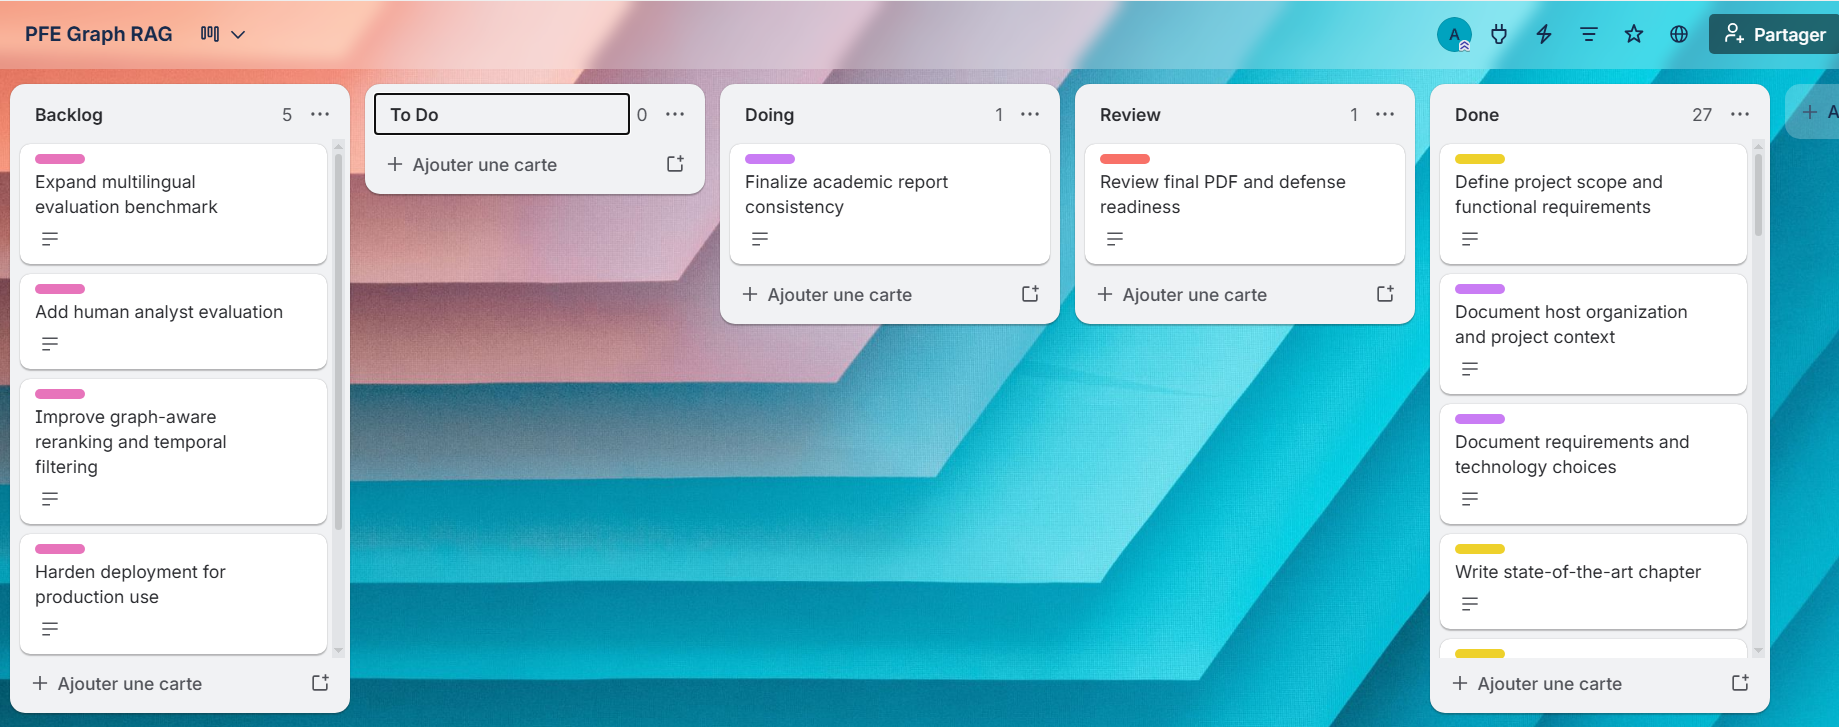
\includegraphics[width=\textwidth,height=0.82\textheight,keepaspectratio]{images/kanban.png}
    \caption{Trello Kanban board used to manage the project workflow.}
    \label{fig:kanban-workflow}
\end{figure}

Trello supported the continuous organization, prioritization, monitoring, and
validation of project activities. Moving cards across the workflow made the
current state of work visible and ensured that validation remained integrated
into development rather than being postponed until the end of the project.

\subsubsection{Project Management Tools}

Modern agile teams often implement Kanban and communication practices through dedicated platforms. During the end-of-study internship, \textbf{Trello} provided the visual board for story cards, column transitions, due dates, and checklist-based acceptance criteria, while \textbf{Slack} supported synchronous coordination, file sharing, and rapid escalation when blockers affected ingestion or model access. Figure~\ref{fig:pm-tools} identifies these tools as representative of contemporary project-management practice; they do not alter the requirement baseline itself but make task ownership, status, and review cycles auditable across the three-month timeline.

\begin{figure}[H]
    \centering
    \raisebox{-0.15\height}{
\includegraphics[height=0.95cm]{Logos/trello.pdf}}\hspace{1.2cm}
    \raisebox{-0.15\height}{
\includegraphics[height=0.95cm]{Logos/slack.pdf}}
    \caption{Trello (Kanban board) and Slack (team communication) used to manage internship tasks and coordination.}
    \label{fig:pm-tools}
\end{figure}

Trello translated each user story into a trackable card with assignee, labels (for example ingestion, retrieval, or frontend), and definition-of-done checklists. Slack complemented the board by documenting decisions that were too granular for card updates---API key provisioning, corpus expansion priorities, or demo feedback---so that requirement changes remained traceable without polluting the formal requirement tables in this chapter.

\subsubsection{Execution Timeline (Gantt Diagram)}

Figure~\ref{fig:pfe-project-execution-gantt} presents a \textbf{Gantt diagram} of the project execution timeline aligned with major requirement delivery milestones. Gantt charts express parallel and sequential activities on a shared calendar axis; they complement Kanban boards by showing \emph{when} macro-phases occur, whereas Kanban shows \emph{what} is currently in flight and \emph{who} owns each item.

\begin{figure}[H]
    \centering
    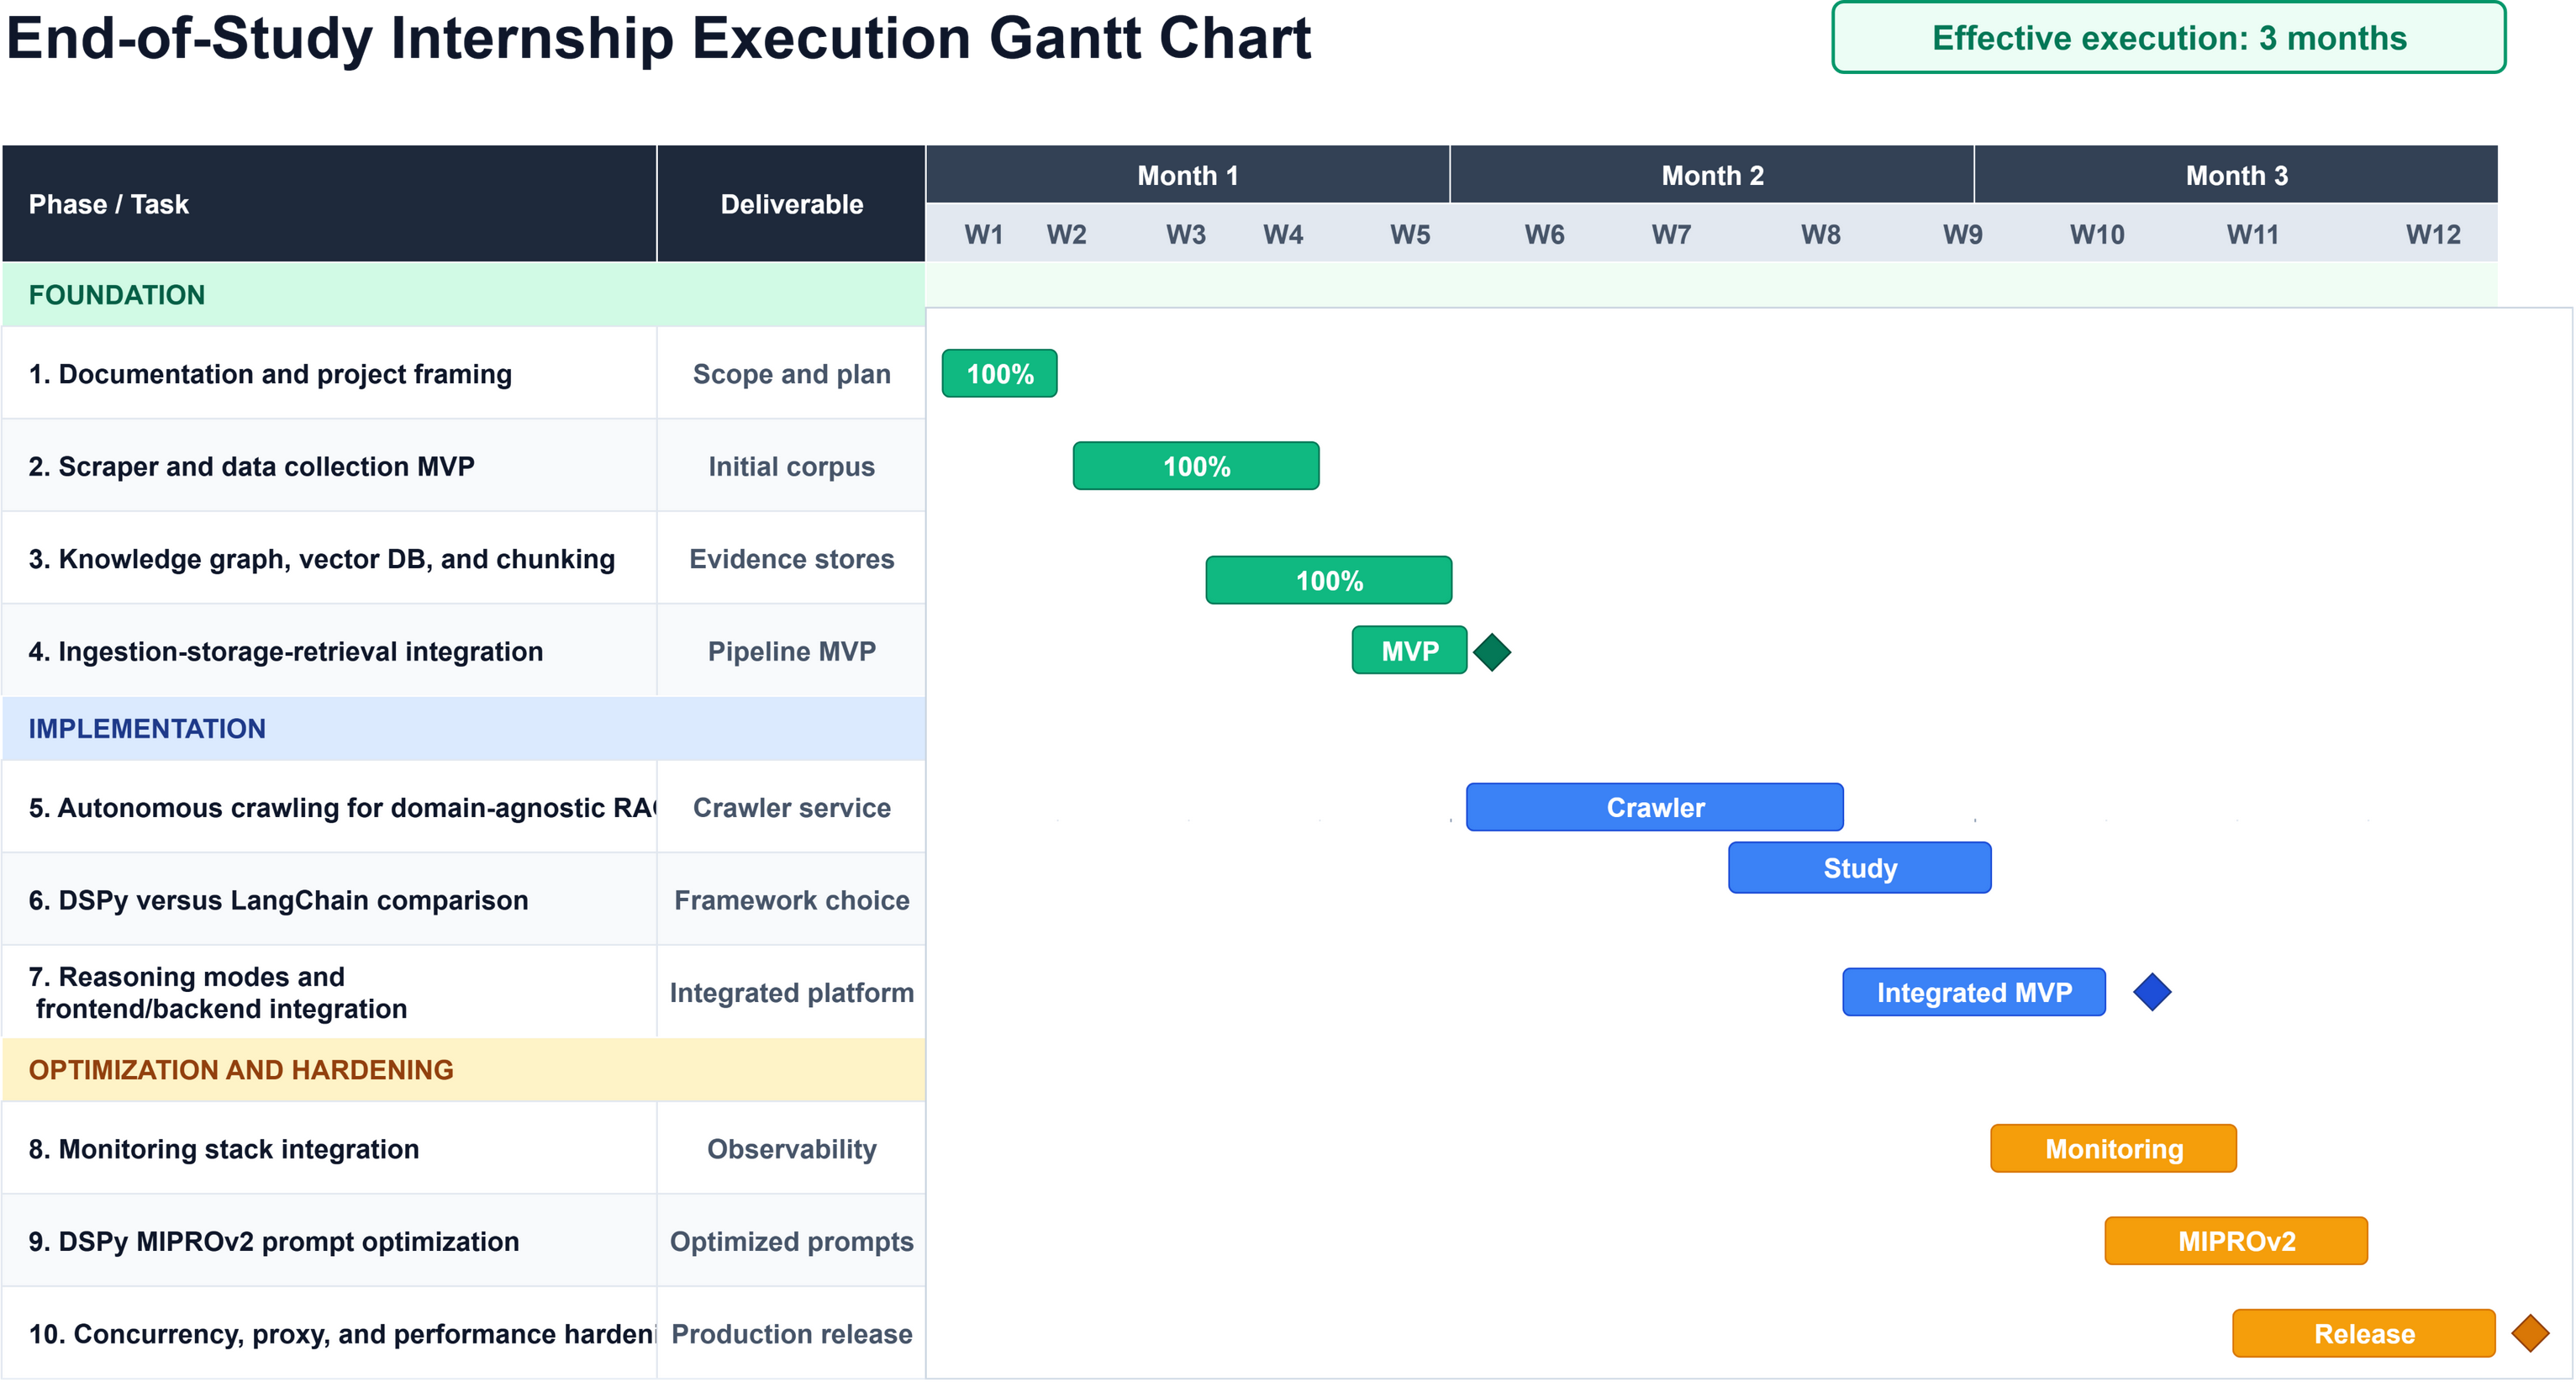
\includegraphics[width=\textwidth,height=0.82\textheight,keepaspectratio]{images/pfe_project_execution_gantt_diagram.png}
    \caption{Gantt diagram of the end-of-study internship timeline aligned with major requirement delivery milestones.}
    \label{fig:pfe-project-execution-gantt}
\end{figure}

The structured Gantt chart organizes the work into foundation, implementation, and optimization phases across twelve weekly columns. The task bars show that project framing, corpus acquisition, knowledge-graph construction, vector indexing, and the first integrated retrieval pipeline occupied the initial month. Autonomous crawling, framework comparison, and the integration of the three reasoning modes followed during the second month. The final month concentrated on observability, MIPROv2 prompt optimization, concurrency, proxy configuration, and performance hardening. Dependency arrows make the delivery order explicit, while milestone markers identify the pipeline MVP, the integrated analytical platform, and the production-ready release. This sequencing ensured that evaluation and optimization were performed only after the evidence stores and end-to-end query path had reached a stable state.

\section{Requirements Validation Criteria}

\subsection{Evidence and Metrics}

Operational validation was organized by requirement area. For each area, a criterion states what must be demonstrably true before the area is accepted; the expected evidence lists the artifacts that prove compliance during development and acceptance testing. Quantitative scores (lexical overlap, semantic similarity, RAGAS-style metrics) are reported in Chapter~5 against a curated benchmark; the criteria here define minimum observable outcomes during implementation.

\textbf{Ingestion.} New sources and formats must be processable without modifying the reasoning engine. Evidence includes ingestion logs, normalized MongoDB document records, and scheduler status visible from the administration dashboard. This criterion verifies modularity between acquisition and downstream analytics.

\textbf{Extraction.} Entities and relations must conform to the target schema and publish cleanly to Neo4j. Evidence includes structured JSON outputs, typed nodes and edges, and rejection or repair logs when parsing fails. Structural correctness is validated before answer-quality metrics are interpreted.

\textbf{Retrieval.} Queries must return both semantic chunks and, when applicable, graph paths supporting the question. Evidence includes ZVec hit lists, Neo4j traversal results, and citation metadata attached to retrieved evidence.

\textbf{Reasoning.} Multi-hop and mode-selected questions must yield grounded answers with inspectable traces. Evidence includes reasoning traces, cited synthesis text, and confidence or audit signals exposed in the chat interface.

\textbf{Observability.} Pipeline behavior must be inspectable end-to-end under load. Evidence includes Prometheus metrics, Grafana dashboards, and Jaeger distributed traces across ingestion, retrieval, and synthesis services.

Table~\ref{tab:requirements-validation} summarizes these areas in compact form; the narrative above develops each criterion and evidence type in full.

\begin{table}[H]
\centering
\small
\setlength{\tabcolsep}{5pt}
\renewcommand{\arraystretch}{1.35}
\begin{tabularx}{\textwidth}{@{}>{\bfseries\raggedright\arraybackslash}p{2.5cm}>{\raggedright\arraybackslash}X>{\raggedright\arraybackslash}p{3.85cm}@{}}
\toprule
\rowcolor{lightblue}
Requirement area & Validation criterion & Key evidence \\
\midrule
Ingestion & New sources and formats processable without modifying the reasoning engine. & Ingestion logs; normalized MongoDB documents; scheduler dashboard status. \\
Extraction & Entities and relations conform to the target schema and publish to the graph. & Structured JSON outputs; Neo4j nodes and typed edges; rejection or repair logs. \\
Retrieval & Queries return semantic chunks and applicable graph paths for the question. & ZVec hit lists; Neo4j traversal results; citation metadata on evidence. \\
Reasoning & Multi-hop and mode-selected questions yield grounded, cited answers. & Reasoning traces; cited synthesis; confidence or audit signals in the UI. \\
Observability & Ingestion, retrieval, and synthesis behavior inspectable under load. & Prometheus metrics; Grafana dashboards; Jaeger distributed traces. \\
\bottomrule
\end{tabularx}
\caption{Requirements validation criteria by area.}
\label{tab:requirements-validation}
\end{table}

Together, the criteria ensure that ingestion remains modular, that structuring and retrieval are verified before answer-quality evaluation, and that analytical trust rests on inspectable evidence rather than opaque generation alone.

\section{Conclusion}

This chapter presented SCIENTIAE and its need for a reusable Graph-RAG framework, with politics and geopolitics serving as the validation domain. It defined the problem, solution, objectives, actors, UML models, functional and non-functional requirements, technology choices, management approach, and validation criteria. Chapter~2 now reviews the state of the art and positions the proposed framework before Chapter~3 translates these requirements into system architecture and component responsibilities.
